\documentclass[conference]{IEEEtran}
\usepackage[english]{babel}
\usepackage{cite}
\ifCLASSINFOpdf
 \usepackage[pdftex]{graphicx}
 \graphicspath{{./images/}}
 \DeclareGraphicsExtensions{.pdf,.jpeg,.png}
\else
\fi
\usepackage{amsmath}
\newcommand{\argmax}{\operatorname*{argmax}}
\usepackage{array}
\usepackage{url}
\usepackage{hyperref}
\hyphenation{op-tical net-works semi-conduc-tor}
\usepackage{svg}
\usepackage{listings}
\usepackage{xcolor}
\usepackage{subcaption}

\lstset{
  basicstyle=\ttfamily\small,
  backgroundcolor=\color{gray!10},
  frame=single,
  columns=fullflexible,
  keepspaces=true,
  showstringspaces=false
}

\title{Does Functional Similarity Induced by Distillation Preserve Internal Representations and Explanatory Mechanisms in Autoregressive Models?}

\author{
\IEEEauthorblockN{Martín Perciante}
\IEEEauthorblockA{Universidad Católica del Uruguay\\ Montevideo,Uruguay\\\href{mailto:tincho.perciante@gmail.com
}{tincho.perciante@gmail.com}}}

\begin{document}

\maketitle

\begin{abstract}
Knowledge distillation is often evaluated in terms of functional similarity between teacher and student models, typically measured through predictive performance. However, it remains unclear whether this functional similarity also implies the preservation of internal representations and explanatory mechanisms. This work investigates this question in autoregressive Transformer-based models. To this end, a TinyLlama teacher model is distilled into two shallower student models on a generative sentiment classification task, varying the loss function used during training. Internal representations are compared through attention map metrics, spectral analysis, and post-hoc explainability techniques, including \textbf{LIME}, \textbf{SHAP}, and \textbf{Integrated Gradients}. The results show that distillation does not transfer the teacher's explanatory mechanisms, as both students assign importance to tokens lacking sentiment-related content, regardless of their classification performance. Regarding internal representations, a partial transfer of structure is observed in the first-layer attention maps, with Frobenius distances below $2\%$ of the theoretical maximum bound, whereas intermediate and deeper layers exhibit substantial divergences. At a global level, the students attention \textit{rollout} displays high similarity to the teacher's average attention patterns, although this finding requires careful interpretation. Across all analyses, both student models exhibit nearly identical behavior, suggesting that the observed patterns arise from the distillation process itself rather than from the additional $KL$ term applied to class-specific tokens to preserve the logits \textit{argmax}. The absence of a non-distilled baseline prevents definitive conclusions; nevertheless, the empirical results are consistent with the existence of a partial inheritance of internal structure induced by knowledge distillation.
\end{abstract}

\section{Introduction}
Explainable Artificial Intelligence (XAI) encompasses a set of methods and processes aimed at interpreting and explaining the behavior of complex mathematical models. In many application domains, it is essential for deployed systems to be interpretable, enabling the justification of autonomous decisions and fostering user trust.

In recent years, autoregressive models based on the Transformer architecture have revolutionized the field of Natural Language Processing (NLP). Large-scale generative models such as GPT, Claude, and Mistral have demonstrated remarkable capabilities in natural language generation and understanding tasks. Despite their strong performance, these models incur substantial computational costs during both training and inference due to their large number of parameters.

To reduce these costs, several model compression techniques have been proposed, among which knowledge distillation (KD) is one of the most widely adopted. In this approach, a student model is trained to approximate the probability distributions produced by a teacher model, with the goal of reproducing its behavior using a significantly smaller architecture \cite{hinton2015distilling}.

Although distillation aims to preserve the functional behavior of the original model, it remains unclear to what extent the teacher's internal representations and explanatory mechanisms emerge or are reconstructed in the student as a consequence of enforcing similarity in the output distributions. In particular, it is natural to ask whether properties associated with attention mechanisms and prediction explanations are preserved throughout the compression process.

The objective of this work is to investigate the relationship between functional similarity and representational similarity in Transformer models compressed through knowledge distillation. To this end, we consider a generative classification problem \cite{daillm} in which the target classes correspond to single tokens in the teacher model's vocabulary. Within this setting, we analyze and compare both internal representations and explanatory mechanisms of the teacher and student models. The motivation for this study stems from the work of \cite{jain2019attention}, which shows that multiple attention configurations can induce similar predictions, thereby challenging the interpretation of attention as a faithful explanation of model behavior. In this context, we investigate whether enforcing functional similarity through logit-based knowledge distillation is sufficient to induce similarity in the internal representations and attention mechanisms of teacher and student models.

The study combines two complementary levels of analysis. First, we examine properties of internal representations through techniques applied to the model's attention maps. To this end, attention similarity metrics are employed, including cosine similarity, Jensen--Shannon ($JS$) divergence, and matrix norms. In addition, a spectral analysis of the attention maps is performed to characterize and compare their structural properties.

Second, we investigate whether the decisions produced by the student model can be explained in a manner similar to those of the teacher by using post-hoc XAI techniques such as \textbf{LIME} and \textbf{SHAP}, comparing the relevance assigned to different input tokens and features. Gradient-based approaches, including \textbf{Integrated Gradients}, are also employed to study the sensitivity of model predictions with respect to the input. This analysis further enables the evaluation of the explanatory consistency of the student's decisions.

The generated explanations are primarily intended for the technical analysis of models by researchers and practitioners, with the goal of understanding which internal properties emerge under knowledge distillation beyond predictive performance alone. In this way, the present work seeks to provide empirical evidence regarding the extent to which preserving output distributions induces the preservation of internal representations and explanatory mechanisms in compressed models.

\section{Theoretical Background}

\subsection{Transformer-Based Autoregressive Models}

Autoregressive language models constitute a family of probabilistic models designed to predict text sequences by modeling the probability of a token conditioned on the preceding tokens. Given an input sequence $x_1, x_2, ..., x_n$, these models approximate the joint language distribution through an autoregressive decomposition into conditional probabilities, as shown below.

\[
P(x_1, x_2, ..., x_n)
=
\prod_{t=1}^{n}
P(x_t \mid x_{<t})
\]

where the prediction of each token depends exclusively on the preceding context. This paradigm enables iterative text generation by selecting the next token at each step according to the probability distribution learned by the model \cite{bengio2003neural}.

Currently, most large-scale language models are based on the Transformer architecture introduced in \cite{vaswani2017attention}. In particular, models such as GPT, LLaMA, Claude, and Mistral employ \textit{decoder-only} variants, in which processing is performed through causal self-attention mechanisms. This constraint ensures that each token can only access information from previous positions in the sequence, thereby preserving the autoregressive behavior of the model.

The Transformer architecture replaces traditional recurrent mechanisms with blocks composed primarily of attention mechanisms, residual connections, and feed-forward neural networks. Attention enables the model to assign different levels of relevance to input tokens, facilitating the capture of both local and long-range dependencies within text. In autoregressive models, this mechanism is implemented causally, preventing a token from attending to future positions during inference.

Modern language models typically consist of multiple Transformer blocks stacked sequentially, allowing progressively more abstract representations of the input text to be constructed. Each block incorporates multi-head attention mechanisms, where different attention heads may specialize in specific linguistic patterns, syntactic relationships, or semantic dependencies. This hierarchical organization has proven highly effective for complex natural language processing tasks.

In addition to text generation, autoregressive models can be adapted to classification tasks through an approach known as \textit{generative classification} \cite{daillm}. In this paradigm, the classification problem is reformulated as a constrained generation task, in which the model is required to produce a token or sequence of tokens corresponding to a predefined class. Unlike architectures specifically designed for classification, where the final layer is typically replaced by a classifier adapted to the number of classes, generative classification preserves the model's original vocabulary space, and predictions are obtained from the logits associated with the target classes.

This approach offers several methodological advantages for the present work. By preserving the model's original generative architecture, it becomes possible to study internal mechanisms such as attention maps, activations, and probability distributions without substantially modifying the structure of the teacher model. Furthermore, it enables distillation procedures to be applied directly to full vocabulary distributions, maintaining consistency with the original training objective of language models.

\subsection{Knowledge Distillation}

Knowledge distillation is a model compression technique whose objective is to transfer information from a high-capacity model, referred to as the teacher, to a smaller or more efficient model, referred to as the student \cite{hinton2015distilling}. This approach seeks to reduce the computational requirements associated with training and inference while preserving part of the performance achieved by large-scale models.

In its traditional formulation, distillation consists of training the student not only on the ground-truth labels of the dataset, but also on the probability distributions produced by the teacher. These distributions contain additional information about relationships between classes, model uncertainty, and implicit semantic similarities. For example, in a classification problem, even when one class is correct, the teacher may assign non-negligible probabilities to related classes, thereby providing richer training signals than conventional discrete labels.

Knowledge transfer is typically implemented through a combination of a standard \textit{cross-entropy} term and a distribution-matching term based on the Kullback--Leibler ($KL$) divergence. The $KL$ divergence measures the discrepancy between a distribution and a reference distribution and is inherently asymmetric. In the context of distillation, this asymmetry is desirable, since the objective is precisely for the student to approximate the behavior of the teacher, which remains fixed during training.

To enrich the information being transferred, a distillation temperature $T$ is often applied to the logits of both models before probabilities are computed using the softmax function. Temperatures greater than $T=1$ produce softer distributions, reducing the dominance of the most probable classes and making it possible to observe more subtle relationships among alternatives. This mechanism encourages the student to learn structural decision patterns present in the teacher beyond the final prediction itself. In the limiting case of $T \rightarrow 0$, the distribution collapses to the most probable token, effectively turning the model into a deterministic text generator.

Knowledge distillation has been widely employed in deep neural networks and, more recently, in large language models, where the computational costs associated with training and inference are particularly high. Most existing work evaluates the success of distillation primarily in terms of functional metrics, such as accuracy or loss on evaluation datasets \cite{gou2021knowledge}.

\subsection{Explainable Artificial Intelligence}

Explainable Artificial Intelligence (XAI) encompasses a set of techniques and methodologies aimed at interpreting, justifying, and understanding the behavior of complex machine learning models. Its primary objective is to provide explanations of how a model arrives at a particular decision, thereby promoting transparency, trust, and interpretability in systems that would otherwise operate as black boxes.

The need for explainability is particularly evident in domains where automated decisions have significant consequences, such as healthcare, finance, law, and recommendation systems. In these contexts, achieving high predictive performance is not sufficient; understanding the factors that drive a model's decisions is equally important. More generally, XAI techniques enable the study of the internal mechanisms of complex models, facilitating the analysis of errors, biases, and emergent behaviors.

Explainability methods can be categorized in several ways. A common distinction separates intrinsically interpretable methods from \textit{post-hoc} methods. The former correspond to models whose structure is naturally understandable, whereas the latter seek to generate explanations for already-trained complex models without modifying their original architecture. Since the Transformer models considered in this work are highly complex and contain a large number of parameters, the present study focuses primarily on post-hoc explainability methods.

\subsubsection{Model-Agnostic Methods}

Model-agnostic methods are explainability techniques that do not require access to the internal structure or parameters of a model. Instead, they operate solely by observing the relationship between inputs and outputs, treating the model as an arbitrary prediction function. This property makes them applicable to a wide range of architectures without requiring model-specific modifications.

One of the most widely used approaches in this category is \textbf{LIME} \cite{ribeiro2016should}. This method seeks to locally approximate the behavior of a complex model using a simpler and more interpretable surrogate model, typically a linear model. To achieve this, perturbations are generated around the original input and the resulting variations in the model output are analyzed, allowing the relative importance of different features to be estimated. In natural language processing tasks, \textbf{LIME} is commonly applied by perturbing words or tokens in a text and observing how their presence or absence affects the prediction.

Another widely adopted method is \textbf{SHAP} \cite{lundberg2017unified}, which is based on cooperative game theory. \textbf{SHAP} assigns an individual contribution to each input feature through Shapley values, interpreting the prediction as the outcome of cooperation among features. In text-based applications, these values make it possible to estimate how much each word or token contributes to the model's final prediction. Compared with other approaches, \textbf{SHAP} provides desirable theoretical properties such as consistency and additivity, although typically at a higher computational cost.

\subsubsection{Gradient-Based Methods}

Gradient-based methods exploit the differentiability of deep neural networks to estimate the influence of input features on model predictions. In general, these techniques evaluate how small changes in the input affect the model output, thereby identifying the components that are most relevant to a particular decision.

Among the simplest approaches are \textit{saliency maps}, which are constructed from the gradient of the model output with respect to the input. The magnitude of the gradient can be interpreted as a measure of sensitivity: features whose variations induce substantial changes in the prediction are considered more relevant to the model's decision.

However, raw gradients can be unstable and may suffer from saturation issues, particularly in regions where small changes in the input produce either abrupt or negligible changes in the model output. To address these limitations, \textbf{Integrated Gradients} \cite{sundararajan2017axiomatic} computes attributions by integrating gradients along a continuous path between a reference input (\textit{baseline}) and the actual input.

\[
\mathrm{IG}_i(x)
=
(x_i - x_i')
\int_0^1
\frac{
\partial F\left(x' + \alpha(x-x')\right)
}{
\partial x_i
}
d\alpha
\]

where $x$ denotes the actual input, $x'$ the reference input, $F(\cdot)$ the model function whose prediction is to be explained, and $\alpha \in [0,1]$ parameterizes the interpolation path between the two inputs. In practice, the integral is approximated by a discrete summation over multiple interpolated points between the \textit{baseline} and the input.

\[
\mathrm{IG}_i(x)
\approx
(x_i - x_i')
\frac{1}{m}
\sum_{k=1}^{m}
\frac{
\partial F\left(
x' + \frac{k}{m}(x-x')
\right)
}{
\partial x_i
}
\]

where $m$ denotes the number of steps used to approximate the integral.

In natural language processing tasks, gradient-based methods make it possible to quantify which tokens have the greatest influence on the probability assigned to specific outputs. In particular, attributions are typically computed with respect to the input embeddings, allowing the relative contribution of each token to the model's prediction to be estimated.

\subsubsection{Attention-Based Methods and Internal Representations}

Unlike purely post-hoc methods that explain decisions solely through perturbations or gradients, Transformer models provide potentially interpretable internal mechanisms through \textit{attention maps}. These maps represent how each token distributes its attention across other positions in the sequence during information processing.

For each attention head and layer, self-attention mechanisms generate matrices that quantify dependency relationships between tokens. Intuitively, these matrices make it possible to observe which parts of the input are used to construct internal representations at different stages of processing. Several studies have suggested that specific attention heads may specialize in syntactic patterns, semantic relationships, or contextual dependencies.

Nevertheless, the use of attention as an explanatory mechanism remains a matter of debate \cite{jain2019attention, wiegreffe2019attention}. Some authors argue that attention does not necessarily provide a causal explanation of model behavior, since the final representations also depend on feed-forward components, residual connections, and intermediate normalization layers. As a result, the direct interpretation of individual attention maps may be insufficient to fully characterize the decision-making process.

To address this limitation, techniques such as \textit{Attention Rollout} \cite{abnar2020quantifying} have been proposed. The objective of this approach is to model the cumulative propagation of information across multiple attention layers. Rather than analyzing individual attention matrices in isolation, this method successively combines attention patterns across layers while incorporating the effect of residual connections, thereby providing a more global approximation of how information flows from input tokens to later representations.

\subsection{Comparison Metrics for Attention Maps}

Attention maps can be interpreted as structured representations of token dependencies, where each row describes a probability distribution over the attended context. This makes it possible to compare representations across models using geometric, matrix-based, and probabilistic metrics in order to quantify structural similarities and differences in the learned attention patterns. In this work, we employ complementary measures that capture different properties of attention maps, including global alignment, distributional discrepancies, and spectral complexity.

\subsubsection{Cosine Similarity}

Cosine similarity is a widely used measure for comparing vector representations, quantifying the degree of angular alignment between two objects independently of their magnitude. Given two vectorized representations $A$ and $B$, cosine similarity is defined as

\[
\cos(\theta)
=
\frac{
\langle A,B \rangle
}{
\|A\|_2 \|B\|_2
}
\]

where $\theta$ denotes the angle between the vectorized representations $A$ and $B$, $\langle \cdot,\cdot \rangle$ denotes the inner product, and $|\cdot|_2$ denotes the Euclidean norm. By definition, its value is bounded between $-1$ and $1$.

When applied to attention maps, this metric enables the evaluation of structural similarity between attention patterns learned by different models. It is particularly useful for identifying global alignment between representations, even when differences in the scale of the assigned probabilities are present.

\subsubsection{Frobenius Distance}

The Frobenius distance quantifies absolute discrepancies between matrices by considering element-wise differences. Given two attention matrices $A$ and $B$, it is defined as

\[
d_F(A,B)
=
\|A-B\|_F
=
\sqrt{
\sum_{i,j}
(A_{ij}-B_{ij})^2
}
\]

This metric can be interpreted as a matrix generalization of Euclidean distance and is particularly useful for measuring the extent to which two attention maps differ in absolute terms. Unlike cosine similarity, the Frobenius distance is sensitive to variations in scale and magnitude, capturing local differences that may not be reflected solely through geometric alignment. In the context of this work, this measure enables the evaluation of the proximity between attention maps generated by teacher and student models by quantifying global differences in the distribution of attention weights.

Since attention maps are row-stochastic matrices of dimension $n \times n$, the Frobenius distance between two such matrices admits a theoretical upper bound. For each row $i$, the entries $A_{ij}$ and $B_{ij}$ are non-negative and sum to $1$.

\[
\sum_j (A_{ij} - B_{ij})^2 
\leq 
\sum_j A_{ij}^2 + \sum_j B_{ij}^2 
\leq 
\sum_j A_{ij} + \sum_j B_{ij} = 2
\]

where we used the fact that $x^2 \leq x$ for $x \in [0,1]$. Summing over the $n$ rows yields

\[
d_F(A,B)^2 = \sum_{i,j}(A_{ij}-B_{ij})^2 \leq 2n
\]

and therefore

\[
d_F(A,B) \leq \sqrt{2n}
\]

This bound is attained when each row of $A$ and $B$ concentrates all its probability mass on different tokens. For $n \times n$ attention maps with $n = 2048$, the maximum possible value is $\sqrt{2 \cdot 2048} = 64$.

\subsubsection{Jensen-Shannon Divergence}

Since the rows of attention maps can be interpreted as probability distributions over tokens, it is natural to employ information-theoretic measures to compare representations. In this work, we use the Jensen--Shannon ($JS$) divergence, a symmetric and bounded measure derived from the $KL$ divergence.

For two probability distributions $P$ and $Q$, the $JS$ divergence is defined as

\[
JS(P,Q)
=
\frac{1}{2}
D_{KL}(P\|M)
+
\frac{1}{2}
D_{KL}(Q\|M)
\]

where

\[
M
=
\frac{1}{2}(P+Q)
\]

denotes the average distribution of $P$ and $Q$.

Unlike the Kullback--Leibler divergence, $JS$ is symmetric and bounded, taking values in the interval $[0,\ln 2]$ when measured in nats, where $0$ corresponds to identical distributions and $\ln 2$ corresponds to distributions with disjoint support. These properties make it particularly suitable for comparing attention distributions \cite{lin1991divergence}.

\subsubsection{Effective Ranks}

Beyond direct comparisons between attention maps, global properties of representations can be characterized through spectral analysis. Using decompositions such as the \textit{Singular Value Decomposition} (SVD), the singular values associated with attention matrices can be analyzed, making it possible to study how information is distributed across different directions of the representational space.

In this context, the concept of \textit{effective rank} provides a measure of the functional dimensionality of a representation, taking into account not only the algebraic rank of the matrix but also the relative concentration of energy in its principal components. Rather than assuming that all dimensions contribute equally, these measures estimate how many spectral directions participate significantly in the representation.

To quantify the geometric complexity of attention maps, two complementary definitions of effective rank were employed. The first corresponds to the entropy-based effective rank (\textit{Entropy Rank}), defined in terms of the Shannon entropy of the normalized singular values \cite{roy2007effective}.

\[
ER
=
\exp
\left(
-\sum_i p_i \log p_i
\right),
\qquad
p_i
=
\frac{\sigma_i}{\sum_j \sigma_j}
\]

where $\sigma_i$ denotes the $i$-th singular value of the matrix.

Additionally, an energy-based definition known as the \textit{Participation Ratio} ($PR$) was employed \cite{recanatesi2022scale}.

\[
PR
=
\frac{
\left(
\sum_i \sigma_i^2
\right)^2
}{
\sum_i \sigma_i^4
}
\]

This metric estimates how many spectral components contribute significantly to the representation while penalizing distributions that are highly concentrated in a small number of dominant directions. The combined use of both measures enables the analysis of similarities and differences between representations from complementary perspectives on the structural complexity of attention mechanisms.


\section{Methodology}

The project was developed in \textbf{Python}, due to its widespread adoption within the scientific community and the availability of specialized tools for deep learning and XAI techniques. Model implementation and training were carried out using \textbf{PyTorch}, together with Hugging Face's \textbf{transformers} library for loading and manipulating language models. In addition, \textbf{NumPy} and \textbf{Pandas} were used for data processing and manipulation, \textbf{Matplotlib} for result visualization, and the \textbf{lime} and \textbf{shap} libraries for explanatory analysis of model predictions. Finally, \textbf{scikit-learn} was employed to compute performance metrics and evaluate the models on the \textbf{test} dataset.

The teacher model used in this work was \textbf{TinyLlama-1.1B-Chat-v1.0}. This model is an autoregressive Transformer decoder-only architecture \cite{vaswani2017attention} composed of $22$ Transformer layers. Its design aims to preserve a structure similar to larger models from the LLaMA family while significantly reducing the number of parameters and the computational cost associated with training and inference. The model incorporates modern attention mechanisms, RMSNorm normalization, and rotary positional embeddings, following an architecture representative of contemporary language models \cite{zhang2024tinyllama}.

To maintain comparability between the internal representations of the teacher and student models, the student architecture preserved the same embedding configuration, attention mechanisms, and hidden dimensions, reducing only the depth of the network. Specifically, the number of Transformer blocks was reduced from $22$ to $11$, resulting in a $2:1$ correspondence between teacher and student blocks and facilitating layer-wise comparisons.

\begin{figure}
\centering
\includesvg[scale=0.7]{./images/architecture_design.svg}
\caption{Comparison between the teacher model architecture (left) and the student model architecture (right). The student is initialized entirely with random weights and inherits no parameters from the teacher. Each internal layer of the student has the same size and architecture as the corresponding layers of the teacher.}
\label{architecture_reduction}
\end{figure}

When using a generative language model for binary classification, several challenges arise. First, the natural output of the model corresponds to a distribution over the entire vocabulary, which contains $32000$ tokens in the selected teacher model, whereas the task requires only two possible classes. Furthermore, generated tokens do not necessarily coincide with the expected class labels. To address this issue, we verified that the classification labels could be represented by a single token in the model vocabulary (\textit{positive} and \textit{negative}). During training, the loss function was computed over the complete vocabulary distribution, preserving the model's original autoregressive behavior. However, for classification and evaluation purposes, only the logits associated with the target tokens were considered, and the prediction was interpreted as the class with the highest relative probability among them, regardless of whether these tokens were the most probable tokens in the full vocabulary \cite{daillm}.

When working with autoregressive models, the classification problem must be adapted to the generative paradigm used by the model. To achieve this, a base prompt containing a placeholder for the dataset input text was defined, while the expected output consisted of the same prompt concatenated with the target class label. During training, a loss mask was applied so that only the target class token contributed to the loss function. In this way, the model was trained under a generative classification framework restricted to a single target output.

\begin{lstlisting}
Review: {input}
Summary:
\end{lstlisting}

For this study, we used the IMDb sentiment analysis dataset, which consists of $50000$ balanced movie reviews labeled with positive or negative sentiment \cite{lopez2019imdb}. Since the teacher model has a maximum context window of $2048$ tokens, the dataset inputs were filtered to ensure that the prompt concatenated with the target label did not exceed this limit. The filtered dataset ($49987$ valid examples) was then split into \textbf{train}, \textbf{validation}, and \textbf{test} sets, resulting in final sizes of $22492$, $2500$, and $24995$ examples, respectively.

The teacher model corresponds to a language model pretrained for text generation tasks \cite{zhang2024tinyllama}. However, the task considered in this work differs from its original objective. For this reason, a fine-tuning process was performed using a single epoch of the \textbf{train} set, with a \textbf{learning rate} of $2 \times 10^{-5}$, batch size equal to $1$, and the \textbf{AdamW} optimization algorithm. All remaining optimizer parameters were left at their default values. Cross-entropy loss computed over the complete vocabulary was used as the training objective. Fine-tuning was performed over all model parameters.

To avoid overfitting and unnecessary training, \textbf{early stopping} was applied, halting training if model performance failed to improve after $5$ consecutive validation rounds. Validation was performed on random subsets of size $100$ sampled from the \textbf{validation} dataset. During each validation step, training checkpoints were stored to enable recovery from failures, together with the model weights corresponding to the lowest validation loss observed up to that point.

The student model was randomly initialized and trained for $3$ epochs on the \textbf{train} set without applying \textbf{early stopping}. The same batch size and optimization algorithm used for the teacher were retained, while the \textbf{learning rate} was increased to $1 \times 10^{-4}$ because training started from random initialization. The \textbf{validation} set was used solely for checkpointing and for storing the weights corresponding to the best-performing model observed during training.

The loss function combined a supervised cross-entropy term with a distillation term based on the $KL$ divergence between the teacher and student probability distributions, encouraging both task learning and functional similarity to the teacher. The total loss was defined as

\[
\mathcal{L}
=
\frac{1}{2}\mathcal{L}_{CE}
+
\frac{1}{2}T^2
D_{KL}(P_P \Vert P_S)
\]

where $\mathcal{L}_{CE}$ denotes the supervised cross-entropy term, $D_{KL}(P_P \Vert P_S)$ represents the $KL$ divergence between the probability distributions generated by the teacher ($P_P$) and the student ($P_S$), and $T$ is the distillation temperature. Equal weighting was assigned to both terms through coefficients of $1/2$. To enrich the information transferred from the teacher, a distillation temperature of $T=2$ was employed, and the distillation term was additionally scaled by $T^2=4$ to preserve gradient magnitudes, following the original distillation formulation proposed in \cite{hinton2015distilling}.

Both the fine-tuned teacher and the student model were evaluated on the \textbf{test} set before comparisons were conducted. This evaluation was performed to verify the correct operation of the models and their expected behavior on the task. Since the problem corresponds to generative classification with a single output token, the models were evaluated using a single forward pass and analyzing the logits of the target classes. This approach is computationally less expensive than using the full generative decoding loop and also avoids generating tokens outside the expected class set. Consequently, the comparison was restricted to the logits associated with the target classes. The final prediction was obtained by selecting the class corresponding to the highest logit among the target tokens. After classifying all examples, the metrics \textit{accuracy}, \textit{precision}, \textit{recall}, \textit{F1-score}, and the confusion matrix were computed.

A limitation emerged from the original distillation objective. The $KL$ divergence between teacher and student is a global measure over the entire vocabulary distribution. As a consequence, two models may exhibit similar distributions overall without necessarily preserving the relative probability ordering within a specific subset of tokens. In the context of this work, this implies that the most probable class token may differ between teacher and student even when the global distributions are highly similar.

To mitigate this issue, a second student model with the same architecture was trained, modifying only the loss function. In addition to the cross-entropy and global distillation terms, an auxiliary $KL$ divergence term was incorporated and computed exclusively over the logits associated with the class tokens. The resulting loss function is given by

\[
\mathcal{L}
=
\frac{1}{2}\mathcal{L}_{CE}
+
\frac{1}{2}T^2D_{KL}(P_P \Vert P_S)
+
\frac{1}{4}T^2D_{KL}(P_P^{(c)} \Vert P_S^{(c)})
\]

where $P_P^{(c)}$ and $P_S^{(c)}$ denote the probability distributions restricted to the \textit{positive} and \textit{negative} tokens. The original weighting between the supervised and global distillation terms was preserved, while the new term was incorporated as an auxiliary signal with lower relative influence during optimization. In particular, it was assigned a smaller weight so as to act as a complementary regularization term, reinforcing the transfer of task-specific knowledge without overriding the distributional information captured by global distillation. Consequently, the new optimization objective seeks not only to approximate the full vocabulary distributions between teacher and student, but also to preserve the relative probability ordering of the classes relevant to the classification task.

After verifying the correct operation of the models on the \textbf{test} set, comparisons of outputs and internal representations were performed between the teacher and both student models. Functional evaluation was conducted using classical post-hoc XAI methods, namely \textbf{LIME}, \textbf{SHAP}, and \textbf{Integrated Gradients}, with the objective of identifying which words or tokens exert the greatest influence on classification decisions. The resulting explanations were then used to compare the degree of explanatory consistency between the teacher and student models.

These methods were applied to two examples from the dataset, one with positive sentiment and one with negative sentiment. For \textbf{LIME}, the \textbf{LimeTextExplainer} was used, generating random perturbations of the input text by removing complete words and observing the resulting variations. For \textbf{SHAP}, text masking was employed, producing a similar procedure based on hiding words from the input text. \textbf{Integrated Gradients} was implemented using the model's \textit{padding token} as the baseline and analyzing how different tokens affected the output. For consistency with the other methods, token-level attribution scores were aggregated after reconstructing complete words.

The output probability distributions of the teacher and student models were compared at temperatures $T=1$ and $T=2$, considering only the global vocabulary distributions. These temperatures were selected because $T=1$ corresponds to standard inference and $T=2$ was used during distillation training. The objective of this analysis was to assess the probabilistic similarity of the predictions beyond the final predicted label. In this way, the study evaluates the extent to which both models exhibit similar distributional behavior, even in cases where their point predictions differ.

Comparisons of internal representations focused on similarities and differences in attention mechanisms beyond the importance assigned to individual tokens. Experiments were conducted using two complementary perspectives: a microscopic (granular) analysis and a macroscopic (global) analysis. The granular approach compared teacher attention blocks with potentially corresponding layers in each student model. More specifically, attention map $i$ of each student was compared with either the average attention map or the attention rollout obtained from teacher layers $2i$ and $2i+1$. This comparison is enabled by the $2:1$ architectural relationship between teacher and student models. The global approach focused on comparing the average attention maps and attention rollouts of the complete models. All comparisons were performed on attention maps averaged over the \textbf{test} dataset rather than on individual examples. At the representational level, the goal was to characterize the average behavior of the models regardless of the analysis scale. Additional comparisons between the two student models were also conducted to identify common structural patterns.

Multiple metrics were employed for attention-block comparisons. First, the matrices were vectorized and cosine similarity was computed to measure the alignment of attention representations within a vector space. Frobenius distances were also computed, providing a notion of proximity in matrix space. For attention maps, the theoretical upper bound of the Frobenius distance serves as a useful reference, although it does not strictly apply to attention rollouts. Since attention maps define a probability distribution on each row by construction, the $JS$ divergence can be naturally used to compare rows between attention blocks. The row-wise $JS$ divergences were averaged, yielding a metric that compares the average token-level probability distributions represented by different attention blocks.

Beyond distance-based comparisons, spectral properties of the attention blocks were also analyzed in order to study geometric similarities between internal attention mechanisms. To this end, singular values were computed for each attention matrix, and the corresponding $ER$ and $PR$ values were evaluated.

The experiments were conducted using an \textbf{NVIDIA GeForce RTX 5070 Ti} GPU with $16$ GB of \textbf{GDDR7} VRAM. The repository containing the source code and experimental results is available at \textbf{https://github.com/PseudoKiwi/ProyectoXAI}.

The writing of this manuscript was partially assisted by generative language models used exclusively for stylistic revision and textual reformulation tasks: Claude Sonnet 4.6 \cite{anthropic2025claude} (Anthropic) and ChatGPT \cite{openai_chatgpt} (OpenAI).

\section{Results}

\subsection{Compression and Training Times}

The teacher model contains a total of $|P| = 1100048384$ parameters, whereas the student model constructed with half the depth contains $|S| = 615561216$ parameters. This corresponds to a \textit{compression rate}

\[
CR = \frac{|P|}{|S|} \approx 1.787
\]

which is equivalent to an approximate $44\%$ reduction in the number of parameters relative to the teacher model. The parameter reduction is not exactly proportional to the reduction in depth, since components independent of the number of layers, such as the vocabulary embeddings and the output layer (\textit{lm head}), were kept identical between teacher and student in order to preserve representational comparability.

The teacher fine-tuning process required approximately $59$ minutes of training, reaching the \textit{early stopping} criterion before completing the single configured epoch. Evaluation on the \textbf{test} set required approximately $35$ minutes.

For the first student model, distillation training lasted approximately $325$ minutes. The best checkpoint was obtained during the final stages of training, indicating that the model continued to improve until the completion of the configured epochs. Evaluation on the \textbf{test} set required approximately $48$ minutes.

The second student model, trained with the additional distillation term restricted to the target classes, required approximately $329$ minutes of training and $54$ minutes for evaluation on the \textbf{test} set.

\subsection{Evaluation on the \textbf{Test} Set}

Evaluation of the teacher model resulted in an almost perfectly diagonal confusion matrix, with only $798$ out of $24995$ examples being misclassified (Figure~\ref{teacher_cm}). The corresponding metrics are reported in Table~\ref{teacher_metrics}. The model demonstrates strong performance on the generative classification task after fine-tuning.

\begin{figure}[b]
\centering
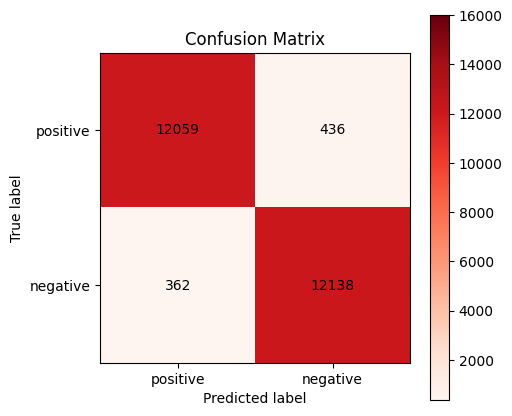
\includegraphics[scale=0.7]{teacher_cm.png}
\caption{Confusion matrix of the teacher model on the generative classification task after fine-tuning, evaluated on the \textbf{test} dataset.}
\label{teacher_cm}
\end{figure}

\begin{table}[h!]
\centering
\caption{Performance metrics of the teacher model on the generative classification task after fine-tuning, evaluated on the \textbf{test} dataset.}
    \begin{tabular}{|c|c|}
        \hline
        Metrica & Value \\ \hline
        Accuracy & $0.9681$ \\
        Precision & $0.9681$ \\
        Recall & $0.9681$ \\
        F1 score & $0.9681$ \\ \hline
    \end{tabular}
    \label{teacher_metrics}
\end{table}

Regarding the first student model, $S_1$, trained under a standard distillation framework, the resulting confusion matrix (Figure~\ref{student_cm}) reveals several issues. First, the total number of misclassified examples is $8203$ out of $24995$. Furthermore, these errors are not uniformly distributed across classes, but instead exhibit a strong bias toward the negative class, with $7997$ out of $12495$ positive examples classified as negative. The corresponding metrics are reported in Table~\ref{student_metrics}. Overall, the performance of $S_1$ is substantially worse than that of the teacher model.

\begin{table}[h!]
\centering
\caption{Performance metrics of the student model on the generative classification task after training, evaluated on the \textbf{test} dataset.}
    \begin{tabular}{|c|c|}
        \hline
        Metric & Value \\ \hline
        Accuracy & $0.6718$ \\
        Precision & $0.7810$ \\
        Recall & $0.6718$ \\
        F1 score & $0.6364$ \\ \hline
    \end{tabular}
    \label{student_metrics}
\end{table}

In contrast to $S_1$, the student model $S_2$ achieves performance close to that of the teacher, resulting in $1643$ misclassified examples out of $24995$. This corresponds to slightly more than twice the number of errors made by the teacher model. The confusion matrix (Figure~\ref{student_local_cm}) reveals a mild bias toward the positive class, as approximately $69\%$ of the misclassified examples were predicted as positive. The corresponding metrics are reported in Table~\ref{student_local_metrics}. Compared with $S_1$, the incorporation of the local $KL$ term is associated with a reduction of approximately $6560$ classification errors and a reversal of the class bias.

\begin{figure}[t]
\centering
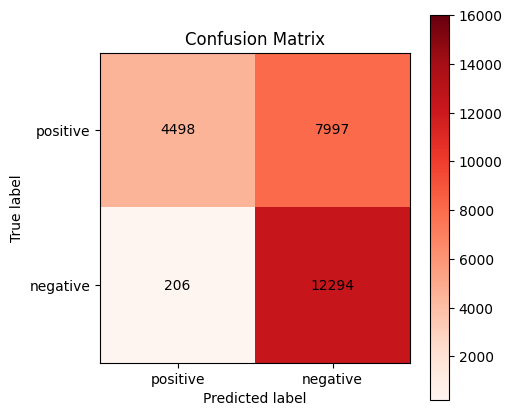
\includegraphics[scale=0.7]{student_cm.png}
\caption{Confusion matrix of the student model on the generative classification task after training, evaluated on the \textbf{test} dataset.}
\label{student_cm}
\end{figure}

\begin{figure}[t]
\centering
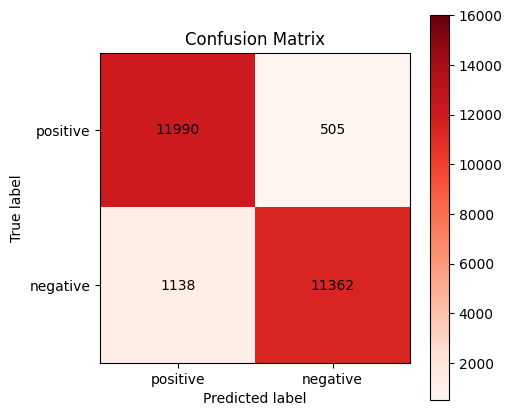
\includegraphics[scale=0.7]{student_local_cm.png}
\caption{Confusion matrix of the student model with local $KL$ distillation on the generative classification task after training, evaluated on the \textbf{test} dataset.}
\label{student_local_cm}
\end{figure}

\begin{table}[h!]
\centering
\caption{Performance metrics of the student model with local $KL$ distillation on the generative classification task after training, evaluated on the \textbf{test} dataset.}
    \begin{tabular}{|c|c|}
        \hline
        Metric & Value \\ \hline
        Accuracy & $0.9343$ \\
        Precision & $0.9354$ \\
        Recall & $0.9343$ \\
        F1 score & $0.9342$ \\ \hline
    \end{tabular}
    \label{student_local_metrics}
\end{table}

Average $KL$ divergence values were computed over the dataset for temperatures $T=1$ and $T=2$. For $T=2$, the results were $KL(P_P \Vert P_{S_1}) \approx 1.1011$ and $KL(P_P \Vert P_{S_2}) \approx 1.5785$, whereas for $T=1$ the values obtained were $KL(P_P \Vert P_{S_1}) \approx 5.8851$ and $KL(P_P \Vert P_{S_2}) \approx 9.2739$. In both cases, $S_1$ exhibits a probability distribution that is closer to $P_P$ according to the global $KL$ divergence. Despite this, the classification metrics of $S_2$ indicate that it is the better model for the task.

\subsection{Functional Evaluation and Comparison}

For the negatively classified example, Figure~\ref{teacher_lime_neg} shows that the teacher model assigns negative weights to words with negative sentiment within the context of the dataset. Similarly, it assigns positive weights to words with positive sentiment. Most of the words identified as important for the prediction receive negative weights and are semantically related to a negative review. This behavior is consistent with the ground-truth class of the example.

In contrast, the explanations produced by both student models differ substantially from that of the teacher (Figure~\ref{student_lime_neg} and Figure~\ref{student_local_lime_neg}). Words such as \textit{and} and \textit{the} receive the highest importance scores despite carrying little or no sentiment-related meaning. A similar pattern can be observed across both student models.

For the positively classified example, Figure~\ref{teacher_lime_pos} shows that the teacher model again assigns negative weights to words with negative connotations and positive weights to words with positive connotations. The resulting explanation is consistent with the class label, which in this case corresponds to a positive review.

\begin{figure}[h!]
\centering

\includegraphics[scale=0.52]{teacher_lime_neg.png}
\caption{\textbf{LIME} explanation generated by the teacher model $P$ for a negative example. The explanation was computed using $5000$ random perturbations of the input text.}
\label{teacher_lime_neg}
\end{figure}

\begin{figure}[h!]
\centering
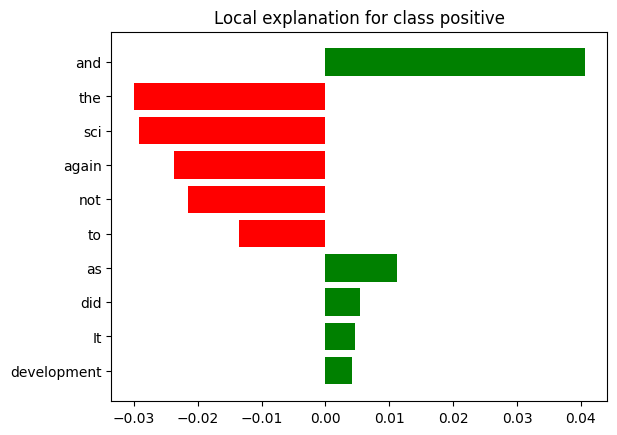
\includegraphics[scale=0.52]{student_lime_neg.png}
\caption{\textbf{LIME} explanation generated by the student model $S_1$ for a negative example. The explanation was computed using $5000$ random perturbations of the input text.}
\label{student_lime_neg}
\end{figure}

\begin{figure}[h!]
\centering
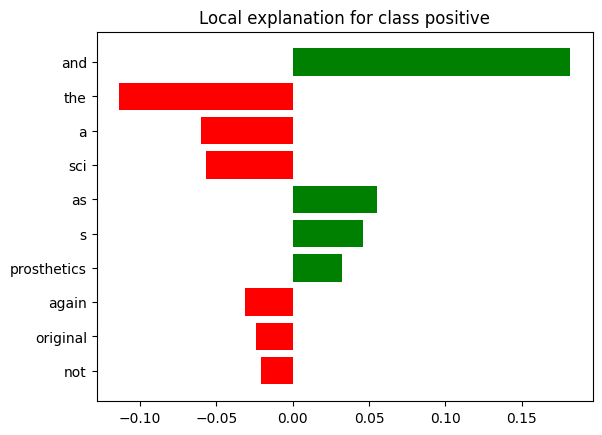
\includegraphics[scale=0.52]{student_local_lime_neg.png}
\caption{\textbf{LIME} explanation generated by the student model $S_2$ for a negative example. The explanation was computed using $5000$ random perturbations of the input text.}
\label{student_local_lime_neg}
\end{figure}

\begin{figure}[h!]
\centering

\includegraphics[scale=0.52]{teacher_lime_pos.png}
\caption{\textbf{LIME} explanation generated by the teacher model $P$ for a positive example. The explanation was computed using $5000$ random perturbations of the input text.}
\label{teacher_lime_pos}
\end{figure}

\begin{figure}[h!]
\centering

\includegraphics[scale=0.52]{student_lime_pos.png}
\caption{\textbf{LIME} explanation generated by the student model $S_1$ for a positive example. The explanation was computed using $5000$ random perturbations of the input text.}
\label{student_lime_pos}
\end{figure}

\begin{figure}[h!]
\centering
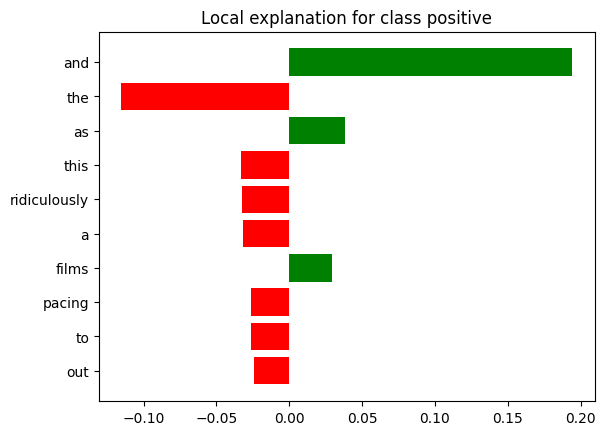
\includegraphics[scale=0.52]{student_local_lime_pos.png}
\caption{\textbf{LIME} explanation generated by the student model $S_2$ for a positive example. The explanation was computed using $5000$ random perturbations of the input text.}
\label{student_local_lime_pos}
\end{figure}

For the student models, the explanations again differ substantially from those of the teacher (Figure~\ref{student_lime_pos} and Figure~\ref{student_local_lime_pos}). The strong attribution assigned to words such as \textit{and} and \textit{the} persists, although the explanations also exhibit notable differences between the two student models.

The results obtained using \textbf{SHAP} and \textbf{Integrated Gradients} are included in Appendix~\ref{anexo:shap} and Appendix~\ref{anexo:ig}, respectively. In the case of \textbf{SHAP}, the teacher model produces attributions that are consistent with the task, whereas the student models predominantly assign importance to words that should not carry such a strong influence given the context. The attributions produced by \textbf{Integrated Gradients} are difficult to interpret for all three models.

The resulting $KL$ divergence values between the students $S_1$, $S_2$, and the teacher $P$ were $KL(P_P \Vert P_{S_1}) \approx 1.1011$ and $KL(P_P \Vert P_{S_2}) \approx 1.5785$ for $T=2$, and $KL(P_P \Vert P_{S_1}) \approx 5.8851$ and $KL(P_P \Vert P_{S_2}) \approx 9.2739$ for $T=1$. In both cases, $S_1$ exhibits a lower $KL$ divergence with respect to the teacher distribution.

\subsection{Representational Comparison}

This section presents the results of the comparisons between the attention maps of the models. We first report layer-wise comparisons and then present the results obtained from global representation comparisons.

\subsubsection{Layer-wise Comparisons}

Tables reporting the results for all the metrics defined to compare attention maps are presented below. We denote by $S_1$ the student trained using standard knowledge distillation, by $S_2$ the student trained with the additional distillation term designed to preserve the argmax among the target-class logits, and by $P$ the teacher model. For each student attention map $i$, comparisons are performed against both the average attention map and the \textit{rollout} obtained from the teacher attention maps $2i$ and $2i+1$.

The cosine similarity between vectorized attention maps is reported in Table~\ref{cosine_similarity}. Overall, comparisons between the students and the teacher exhibit similar trends for both $P_{avg}$ and $P_r$. In the first compared layer ($i=0$), a high similarity is observed between the students and the teacher when using $P_{avg}$, reaching values of $0.9271$ for $S_1$ and $0.9530$ for $S_2$. However, in the second layer ($i=1$), the similarities drop sharply to values close to $0.3$, remaining relatively low throughout intermediate layers and showing only a partial recovery in the deepest layers.

When compared against $P_r$, the overall trends remain similar to those observed with $P_{avg}$, although the first layer exhibits substantially lower values ($\approx 0.28$) than those obtained using the average attention maps. Furthermore, $S_2$ tends to achieve similarities equal to or greater than those of $S_1$ with respect to the teacher in several layers, particularly in the intermediate ones. Finally, the $S_1$--$S_2$ comparison reveals a high degree of similarity between both students across all layers, with values exceeding $0.81$ and, in most cases, approaching $0.9$.

\begin{table}[h!]
\centering
\caption{Cosine similarities between vectorized attention maps of student $S_1$, student $S_2$, and teacher $P$. $S_1$ was trained by minimizing the $KL$ divergence over the full vocabulary with respect to the teacher, whereas $S_2$ additionally incorporates a $KL$ term restricted to the target tokens in order to preserve the argmax. For each student layer $i$, the teacher representations are obtained as the average attention map $P_{avg}$ and the Attention Rollout $P_r$ computed from layers $2i$ and $2i+1$. Comparisons between $S_1$ and $P$, $S_2$ and $P$, and $S_1$ and $S_2$ are reported.}
    \begin{tabular}{|c|c|c|c|c|c|}
        \hline
        $i$ & $S_1-P_{avg}$ & $S_1-P_{r}$ & $S_2-P_{avg}$ & $S_2-P_{r}$ & $S_1-S_2$ \\
        \hline
        0 & $0.9271$ & $0.2752$ & $0.9530$ & $0.2877$ & $0.9713$ \\
        1 & $0.2688$ & $0.2268$ & $0.3106$ & $0.2588$ & $0.9258$ \\
        2 & $0.3348$ & $0.3322$ & $0.5676$ & $0.5316$ & $0.8185$ \\
        3 & $0.1360$ & $0.1484$ & $0.3265$ & $0.3308$ & $0.8940$ \\
        4 & $0.1623$ & $0.1930$ & $0.2454$ & $0.2537$ & $0.9451$ \\
        5 & $0.1579$ & $0.1914$ & $0.3558$ & $0.3669$ & $0.9049$ \\
        6 & $0.1731$ & $0.2138$ & $0.2092$ & $0.2390$ & $0.9586$ \\
        7 & $0.1687$ & $0.2225$ & $0.1995$ & $0.2619$ & $0.9706$ \\
        8 & $0.2197$ & $0.2439$ & $0.2492$ & $0.2897$ & $0.9590$ \\
        9 & $0.2192$ & $0.2334$ & $0.1810$ & $0.2456$ & $0.8860$ \\
        10 & $0.3066$ & $0.3291$ & $0.2851$ & $0.3415$ & $0.8624$ \\
        \hline
    \end{tabular}
    \label{cosine_similarity}
\end{table}

The Frobenius distance between attention maps is reported in Table~\ref{frobenius_distance}. Consistent with the cosine similarity results, the closest attention maps correspond to comparisons against the teacher average attention map in the first layer ($i=0$). It is worth noting that the theoretical maximum Frobenius distance between attention maps of dimension $2048 \times 2048$ is $64$. Consequently, the observed distances, particularly those approaching $40$, represent substantial differences between the compared attention distributions.

\begin{table}[h!]
\centering
\caption{Layer-wise Frobenius distance between attention maps. $S_1$, $S_2$: students; $P_{avg}$, $P_r$: teacher average attention map and \textit{rollout}. Same notation as in Table~\ref{cosine_similarity}.}
    \begin{tabular}{|c|c|c|c|c|c|}
        \hline
        $i$ & $S_1-P_{avg}$ & $S_1-P_{r}$ & $S_2-P_{avg}$ & $S_2-P_{r}$ & $S_1-S_2$ \\
        \hline
        0 & $1.3432$ & $11.3760$ & $1.0846$ & $11.3316$ & $0.8196$ \\
        1 & $18.9485$ & $21.6454$ & $18.7224$ & $21.4776$ & $1.8418$ \\
        2 & $35.8680$ & $30.4318$ & $33.7373$ & $28.6160$ & $4.2136$ \\
        3 & $39.6938$ & $32.8054$ & $38.8643$ & $32.0087$ & $1.9827$ \\
        4 & $25.9925$ & $25.0566$ & $25.6862$ & $24.8451$ & $1.3581$ \\
        5 & $22.6046$ & $23.0084$ & $21.5705$ & $22.1283$ & $2.6141$ \\
        6 & $18.0666$ & $19.9416$ & $17.9186$ & $19.8215$ & $1.4082$ \\
        7 & $17.6782$ & $19.8836$ & $17.5799$ & $19.6842$ & $1.3172$ \\
        8 & $19.0674$ & $20.7777$ & $18.9334$ & $20.5559$ & $1.2321$ \\
        9 & $19.9193$ & $21.3191$ & $20.0786$ & $21.2283$ & $2.0819$ \\
        10 & $20.4072$ & $21.4697$ & $20.4738$ & $21.3467$ & $2.4813$ \\
        \hline
    \end{tabular}
    \label{frobenius_distance}
\end{table}


Moreover, comparisons between $S_1$ and $S_2$ exhibit considerably smaller distances than those observed with respect to the teacher, indicating that both students learn highly similar attention patterns. In general, comparisons against $P_r$ tend to produce larger distances than those against $P_{avg}$ in several layers, particularly in the early ones, although some intermediate-layer comparisons against $P_{avg}$ reach the largest values observed overall.

The row-averaged $JS$ divergence between attention maps is reported in Table~\ref{JS}. Since this metric takes values in the interval $[0,\ln(2)]$, where smaller values indicate more similar distributions, a high degree of agreement between the students and the teacher is observed in the first layer ($i=0$), particularly when compared against $P_{avg}$, yielding values of $0.0122$ for $S_1$ and $0.0086$ for $S_2$.

\begin{table}[h!]
\centering
\caption{Row-averaged $JS$ divergence between attention maps. $S_1$, $S_2$: students; $P_{avg}$, $P_r$: teacher average attention map and \textit{rollout}. Same notation as in Table~\ref{cosine_similarity}.}
    \begin{tabular}{|c|c|c|c|c|c|}
        \hline
        $i$ & $S_1-P_{avg}$ & $S_1-P_{r}$ & $S_2-P_{avg}$ & $S_2-P_{r}$ & $S_1-S_2$ \\
        \hline
        0 & $0.0122$ & $0.1108$ & $0.0086$ & $0.1042$ & $0.0055$ \\
        1 & $0.1646$ & $0.2943$ & $0.1597$ & $0.2893$ & $0.0100$ \\
        2 & $0.3903$ & $0.4644$ & $0.3406$ & $0.4227$ & $0.0327$ \\
        3 & $0.4936$ & $0.5489$ & $0.4627$ & $0.5173$ & $0.0304$ \\
        4 & $0.2674$ & $0.3641$ & $0.2544$ & $0.3564$ & $0.0128$ \\
        5 & $0.2390$ & $0.3247$ & $0.2040$ & $0.2960$ & $0.0225$ \\
        6 & $0.1921$ & $0.2791$ & $0.1812$ & $0.2689$ & $0.0150$ \\
        7 & $0.1894$ & $0.2791$ & $0.1827$ & $0.2678$ & $0.0128$ \\
        8 & $0.2114$ & $0.3001$ & $0.2033$ & $0.2884$ & $0.0126$ \\
        9 & $0.2218$ & $0.3124$ & $0.2221$ & $0.3035$ & $0.0185$ \\
        10 & $0.2148$ & $0.3020$ & $0.2092$ & $0.2924$ & $0.0384$ \\
        \hline
    \end{tabular}
    \label{JS}
\end{table}

In subsequent layers, the divergences increase substantially, reaching their maximum values in intermediate layers ($i=2$ and $i=3$), particularly in comparisons against $P_r$, where values close to $0.55$ are obtained. Thereafter, the divergences decrease and stabilize in deeper layers, although they remain considerably larger than those observed in the first layer.

Furthermore, comparisons between $S_1$ and $S_2$ consistently yield the lowest divergence values across all layers, ranging from $0.0055$ to $0.0384$, indicating a high degree of similarity between the two students. Overall, $S_2$ tends to exhibit divergences equal to or lower than those of $S_1$ with respect to the teacher, particularly in intermediate layers, suggesting a better alignment of its attention patterns.

The $PR$ values computed for each attention map are reported in Table~\ref{participation_ratio}. In general, the maps associated with $P_{avg}$ exhibit values close to $1$ across nearly all layers, suggesting highly concentrated distributions. In contrast, $P_r$ displays markedly different behavior, particularly in the first layer ($i=0$), where it reaches a value of $365.1039$, indicating a substantially more diffuse attention distribution.

\begin{table}[h!]
\centering
\caption{$PR$ computed for each attention map. $S_1$, $S_2$: students; $P_{avg}$, $P_r$: teacher average attention map and \textit{rollout}.}
    \begin{tabular}{|c|c|c|c|c|}
        \hline
        $i$ & $S_1$ & $S_2$ & $P_{avg}$ & $P_{r}$ \\
        \hline
        0 & $2.4352$ & $2.5027$ & $2.9765$ & $365.1039$ \\
        1 & $2.0897$ & $1.7893$ & $1.009$ & $1.8481$ \\
        2 & $1.8754$ & $1.2828$ & $1.0003$ & $1.3134$ \\
        3 & $2.0921$ & $2.1538$ & $1.0005$ & $1.2851$ \\
        4 & $4.1263$ & $3.2787$ & $1.0031$ & $1.5620$ \\
        5 & $8.5767$ & $4.7921$ & $1.0040$ & $1.7202$ \\
        6 & $9.7336$ & $12.6110$ & $1.0109$ & $2.1388$ \\
        7 & $10.1048$ & $15.8588$ & $1.0123$ & $2.1546$ \\
        8 & $4.9535$ & $7.0641$ & $1.0085$ & $1.9760$ \\
        9 & $3.4228$ & $8.6932$ & $1.0055$ & $1.9005$ \\
        10 & $3.2704$ & $8.6830$ & $1.0128$ & $1.8739$ \\
        \hline
    \end{tabular}
    \label{participation_ratio}
\end{table}

In contrast, the student models exhibit values consistently higher than those of $P_{avg}$ and lower than those of $P_r$, with an increasing trend toward intermediate and deeper layers. In particular, $S_1$ and $S_2$ reach their highest values between layers $i=5$ and $i=7$, suggesting an increase in attention dispersion within these representations. Furthermore, differences between the two students emerge in certain layers, especially from $i=6$ onward, where $S_2$ exhibits higher values.

The $ER$ values are reported in Table~\ref{entropy_based}. Unlike $PR$, this metric reveals much more pronounced scale differences between the teacher average attention maps and the teacher \textit{rollout}. While $P_{avg}$ maintains relatively low effective ranks, particularly in early and intermediate layers, $P_r$ consistently exhibits high values, close to $1800$ across all layers, indicating substantially more distributed representations.

\begin{table}[h!]
\centering
\caption{$ER$ computed for each attention map. $S_1$, $S_2$: students; $P_{avg}$, $P_r$: teacher average attention map and \textit{rollout}.}
    \begin{tabular}{|c|c|c|c|c|}
        \hline
        $i$ & $S_1$ & $S_2$ & $P_{avg}$ & $P_{r}$ \\
        \hline
        0 & $77.7460$ & $93.2713$ & $257.7619$ & $2026.0115$ \\
        1 & $75.5660$ & $56.2762$ & $32.7049$ & $1817.4816$ \\
        2 & $137.7758$ & $17.5452$ & $4.4293$ & $1666.9999$ \\
        3 & $159.8630$ & $207.4611$ & $5.7635$ & $1648.0753$ \\
        4 & $354.9870$ & $259.7679$ & $15.9719$ & $1764.5404$ \\
        5 & $534.8630$ & $396.5259$ & $20.1245$ & $1798.4602$ \\
        6 & $400.9078$ & $495.8846$ & $50.6510$ & $1849.4958$ \\
        7 & $419.5436$ & $457.3091$ & $64.9083$ & $1850.6656$ \\
        8 & $348.2325$ & $414.0989$ & $49.0093$ & $1833.6090$ \\
        9 & $298.1621$ & $428.9598$ & $34.7594$ & $1825.2311$ \\
        10 & $382.6713$ & $466.4542$ & $100.7165$ & $1819.1229$ \\
        \hline
    \end{tabular}
    \label{entropy_based}
\end{table}

The student models exhibit an intermediate behavior with respect to the two teacher references, with effective ranks substantially larger than those of $P_{avg}$ but considerably smaller than those of $P_r$. Overall, an increase in effective rank can be observed in deeper layers, particularly from $i=4$ onward. Furthermore, although $S_1$ and $S_2$ follow similar trends, notable discrepancies appear in some layers, such as $i=2$, where $S_2$ exhibits a substantially lower value than $S_1$, and in the final layers, where $S_2$ tends to achieve higher effective ranks.

\subsubsection{Global Comparisons}

The comparison of aggregated global representations is presented in Table~\ref{tab:global_comparison}. Overall, the students' \textit{mean} representations exhibit moderate similarity with respect to the teacher's global average attention representation ($P_{avg}$), achieving cosine similarities of $0.2492$ for $S_1$ and $0.3478$ for $S_2$. Likewise, the $JS$ divergences remain relatively low ($<0.2$), while the Frobenius distances are approximately $21$, indicating partial similarity between the aggregated attention structures.

\begin{table}[h!]
\centering
\caption{Comparison of aggregated global representations using cosine similarity, Frobenius distance, and row-averaged $JS$ divergence. $S_1$ and $S_2$ denote the average attention maps and Attention Rollout computed over all layers of each student. $P$ denotes the teacher average attention maps and Attention Rollout.}
    \begin{tabular}{|l|l|c|c|c|}
        \hline
        Representation A & Representation B & Cosine & Frobenius & JS \\
        \hline
        $S_{1_{avg}}$ & $P_{avg}$ & $0.2492$ & $21.4037$ & $0.1946$ \\
        $S_{1_{avg}}$ & $P_r$ & $0.1731$ & $44.7235$ & $0.6554$ \\
        $S_{2_{avg}}$ & $P_{avg}$ & $0.3478$ & $20.9771$ & $0.1815$ \\
        $S_{2_{avg}}$ & $P_r$ & $0.2693$ & $44.3146$ & $0.6374$ \\
        $S_{1_r}$ & $P_{avg}$ & $0.9534$ & $6.8544$ & $0.1787$ \\
        $S_{1_r}$ & $P_r$ & $0.9434$ & $27.6911$ & $0.2719$ \\
        $S_{2_r}$ & $P_{avg}$ & $0.9773$ & $4.7195$ & $0.1568$ \\
        $S_{2_r}$ & $P_r$ & $0.9699$ & $24.4101$ & $0.2306$ \\
        $S_{1_{avg}}$ & $S_{2_{avg}}$ & $0.9865$ & $0.6835$ & $0.0024$ \\
        $S_{1_{avg}}$ & $S_{2_r}$ & $0.2977$ & $21.2566$ & $0.3120$ \\
        $S_{1_r}$ & $S_{2_{avg}}$ & $0.4221$ & $18.0665$ & $0.2879$ \\
        $S_{1_r}$ & $S_{2_r}$ & $0.9953$ & $3.3768$ & $0.0030$ \\
        \hline
    \end{tabular}
    \label{tab:global_comparison}
\end{table}

On the other hand, the students' \textit{rollout} representations exhibit high similarity with respect to the teacher's global average attention representation, reaching cosine similarities in the range of $0.95$--$0.97$ and considerably smaller Frobenius distances ($4.7195$ and $6.8544$). When compared against the teacher's global \textit{rollout}, cosine similarities remain high ($>0.94$), although the Frobenius distances increase to values close to $24$ and $28$, suggesting that the representations preserve similar global patterns while differing in magnitude or scale.

The comparison between students reveals a high degree of similarity between representations of the same type. In particular, $S_{1_{avg}}$ and $S_{2_{avg}}$ achieve a cosine similarity of $0.9865$, a Frobenius distance of $0.6835$, and a $JS$ divergence of $0.0024$. Similarly, the \textit{rollout} representations of both students reach a cosine similarity of $0.9953$, indicating an almost identical alignment between the learned aggregated attention patterns.

The spectral analysis of the global representations is presented in Table~\ref{tab:spectral_global}. The students' \textit{mean} representations exhibit larger values of both $PR$ and $ER$ than those of the teacher, suggesting a greater dispersion of spectral mass and a broader utilization of effective components. In contrast, the teacher's global representations exhibit $PR$ values close to $1$, indicating a highly concentrated structure.

\begin{table}[h!]
\centering
\caption{Spectral analysis of aggregated global representations. $PR$ and $ER$ are reported for each representation.}
\begin{tabular}{|l|c|c|}
        \hline
        Representation & PR & ER \\
        \hline
        $P_{avg}$ & $1.0052$ & $31.1072$ \\
        $P_r$ & $1.0000$ & $1.0003$ \\
        $S_{1_{avg}}$ & $3.2826$ & $336.6037$ \\
        $S_{1_r}$ & $1.0055$ & $2.4227$ \\
        $S_{2_{avg}}$ & $3.2873$ & $362.2327$ \\
        $S_{2_r}$ & $1.0022$ & $2.1826$ \\
        \hline
    \end{tabular}
    \label{tab:spectral_global}
\end{table}

In particular, the teacher's global \textit{rollout} exhibits both $PR$ and $ER$ values close to $1$, suggesting a representation dominated by very few effective components. The students' \textit{rollout} representations display similar behavior, although with slightly larger values, indicating that aggregation through \textit{rollout} induces substantially more concentrated global representations than those obtained through simple averaging.

\section{Discussion}

\subsection{Evaluation on the \textbf{test} Set}

The strong performance of the teacher model is not surprising. As a general-purpose pretrained model, it is expected to have acquired a basic understanding of language beyond the specific task under consideration. Combined with the fine-tuning process performed to specifically use the class tokens, the obtained results are consistent with expectations. Furthermore, since the positive and negative classes already corresponded to existing tokens in the model's vocabulary, the model was already familiar with their semantic meaning, making them more natural outputs than arbitrary tokens. This may have potentially biased the model toward correct behavior, further reinforced by the fine-tuning process.

In contrast, the student models exhibited substantially different results. In the case of $S_1$, only one of the classes was classified correctly due to a clear bias in its predictions. The poor performance of the model can be attributed to the fact that the $KL$ divergence, when used as a loss function, seeks to produce similar probability distributions but does not preserve the $\argmax$. For the temperature $T=2$ used during training, the average divergence over the dataset was $KL(P_P||P_{S_1}) \approx 1.1011$, indicating that $S_1$ learned the softened distribution produced by $P$ over the entire vocabulary reasonably well.

Nevertheless, for $T=1$, the divergence increases to $KL(P_P||P_{S_1}) \approx 5.8851$, a considerably larger value, reflecting substantial differences in the actual distributions used to select the next token. However, $KL$ divergence does not appear to be a predictive metric of classification performance. Model $S_2$ exhibits $KL(P_P||P_{S_2}) \approx 9.2739$ at $T=1$, corresponding to an even larger divergence, yet its classification results are substantially closer to those of $P$. Even at $T=2$, $S_2$ presents $KL(P_P||P_{S_2}) \approx 1.5785 > KL(P_P||P_{S_1})$, indicating that in neither case does the $KL$ divergence accurately reflect task performance.

Since $S_2$ was trained with an additional term designed to preserve the $\argmax$ of the logits corresponding to the target classes, its classification performance shows a substantial improvement. Nevertheless, it still exhibits a bias in the confusion matrix, with more errors occurring in the classification of negative examples than positive ones. Given that the teacher model does not display this behavior, such bias may be explained by insufficient training, limited data availability, or by the distillation process itself, which, by optimizing over the entire vocabulary, may introduce biases affecting the classification tokens.

\subsection{Functional Evaluation and Comparison}

As discussed previously, since $P$ is a general-purpose pretrained model \cite{cerebras2023slimpajama, zhang2024tinyllama}, it is reasonable to expect that the tokens most relevant to sentiment analysis tasks correspond to those that genuinely convey sentiment information. This is precisely what is observed in the teacher's \textbf{LIME} explanations, both for the positive and negative examples. A similar behavior is observed in the \textbf{SHAP} explanations, where positively connoted words receive positive contributions and negatively connoted words receive negative contributions.

In contrast, both $S_1$ and $S_2$ exhibit explanations that differ substantially from those of $P$. The \textbf{LIME} and \textbf{SHAP} explanations generated for the student models frequently assign high importance to words that carry little or no sentiment information. Across all analyzed examples, the explanations produced by the students cannot be considered satisfactory from a semantic perspective. Despite this, $S_2$ achieves strong predictive performance on the dataset, suggesting that accurate predictions are not necessarily associated with meaningful explanations.

For all models, \textbf{Integrated Gradients} produced results that were difficult to interpret. In most cases, the words receiving the largest attribution scores do not appear to carry sufficient sentiment-related semantic information to justify their importance. This behavior may be related to the choice of the \textit{padding token} as the baseline used for attribution computation.

\subsection{Layer-wise Representation Comparison}

The results obtained from the attention map comparison metrics exhibit a consistent pattern across all evaluated measures: the first layer ($i=0$) systematically shows the highest similarity between the student models and the teacher. For cosine similarity, $S_1$ and $S_2$ achieve values of $0.9271$ and $0.9530$, respectively, when compared against $P_{avg}$, while the $JS$ divergence decreases to $0.0122$ and $0.0086$, and the Frobenius distance is reduced to $1.3432$ and $1.0846$. This behavior is markedly different from that observed in the remaining layers, where all metrics indicate substantially lower alignment with the teacher model.

Since the Frobenius distance between two attention maps of dimension $2048 \times 2048$ is upper bounded by $\sqrt{2 \cdot 2048} = 64$, the observed distances can be interpreted in relative terms. In the first layer, distances of $1.3432$ and $1.0846$ correspond to only $2.1\%$ and $1.7\%$ of the theoretical maximum, indicating an almost complete alignment between the students' attention maps and the teacher average. In contrast, intermediate layers reach distances close to $40$ (for example, $i=3$ with $39.6938$ for $S_1$), corresponding to approximately $62\%$ of the maximum bound and therefore indicating substantial differences. Comparisons against $P_r$ in the first layer yield distances of approximately $11.4$, corresponding to about $18\%$ of the bound, which is still considerably larger than the values obtained against $P_{avg}$.

These results suggest a possible transfer of structural information from the teacher's early attention representations to the student models. One possible interpretation is that deeper layers develop increasingly abstract and teacher-specific representations, making them more difficult to transfer to a model with half the depth, whereas the first layer, which directly processes the input representations, captures more general and transferable patterns. However, it should be noted that this work did not evaluate a non-distilled model with the same architecture as the students. Consequently, it is not possible to rule out the possibility that the observed similarity in the first layer arises from the task and dataset themselves rather than from the distillation process alone.

It is also noteworthy that the high similarity in the first layer is observed in both student models, regardless of whether the training procedure includes the additional token-level $KL$ term. This suggests that, if the phenomenon is indeed a consequence of distillation, it does not depend on the additional loss introduced in $S_2$, but rather on the distillation process itself.

Regarding the effective ranks, both $PR$ and $ER$ reveal that the students consistently occupy an intermediate position between $P_{avg}$ and $P_r$. While $P_{avg}$ exhibits highly concentrated attention distributions, with $PR$ values close to $1$ in most layers and highly variable $ER$ values, $P_r$ produces considerably more dispersed representations, with effective ranks close to $1800$ across all layers while maintaining $PR \approx 2$. The student models, in contrast, display intermediate values that increase toward deeper layers, suggesting that their attention maps are more diffuse than the teacher average but do not reach the level of dispersion characteristic of the rollout representation. This observation is consistent with the fact that rollout accumulates attention across all teacher layers, capturing long-range dependencies that a shallower model cannot directly reproduce. As in the case of the first-layer similarity, determining whether this intermediate behavior is induced by distillation or emerges naturally from the task would require comparison against a non-distilled model of identical architecture.

\subsection{Global Representation Comparison}

The most notable result of the global comparisons is the high similarity between the rollout representations of both students and the global average attention representation of the teacher. Both $S_{1_r}$ and $S_{2_r}$ achieve cosine similarities of $0.9534$ and $0.9773$ with respect to $P_{avg}$, together with Frobenius distances of $6.8544$ and $4.7195$, respectively. These values are substantially lower than those observed in the remaining teacher-student comparisons.

However, this result should be interpreted with caution. Both rollout and average attention representations are row-stochastic matrices, yet they converge toward more uniform distributions through different mechanisms: rollout through the successive multiplication of stochastic matrices, which progressively mixes attention distributions, and averaging through the direct aggregation of individual distributions. Consequently, it cannot be ruled out that part of the observed similarity is an artifact of this convergence toward uniformity rather than a direct consequence of the distillation process itself. Validating this hypothesis would require comparison against the rollout representation of a non-distilled model with the same architecture.

In contrast, the mean attention representations of the students exhibit only moderate similarity with respect to $P_{avg}$, with cosine similarities of $0.2492$ and $0.3478$ for $S_1$ and $S_2$, respectively, and Frobenius distances close to $21$. This indicates that the average attention maps of the students do not faithfully reproduce those of the teacher.

As observed in the layer-wise analysis, both students produce almost identical global representations. The cosine similarity reaches $0.9865$ between the mean representations and $0.9953$ between the rollout representations. This further supports the observation that the additional token-level $KL$ term introduced in $S_2$ does not produce substantial changes in the learned attention patterns.

With respect to the global spectral analysis, the teacher rollout exhibits both $PR$ and $ER$ values close to $1$, indicating an extremely concentrated global representation, consistent with the convergence toward uniformity discussed previously. The student rollout representations display a similar behavior, although with slightly larger values ($ER \approx 2.2$--$2.4$). In contrast, the mean representations of the students exhibit substantially larger effective ranks ($ER \approx 336$--$362$), suggesting that the average of their attention maps utilizes a much broader set of effective components than the teacher, whose global average representation attains an $ER$ of only $31.1$.

\newpage

\section{Conclusions}

This work investigated whether the functional similarity induced by knowledge distillation preserves internal representations and explanatory mechanisms in autoregressive models. Regarding explanations, the results indicate that the answer is generally negative. The student models do not reproduce the teacher's explanatory mechanisms, assigning importance to words without sentimental content regardless of their classification performance. This demonstrates that strong task performance does not imply the transfer of explainability.

With respect to internal representations, the evidence is partial but not discouraging. A transfer of structure is observed in the first-layer attention maps, with Frobenius distances below $2\%$ of the theoretical maximum bound, whereas intermediate and deeper layers exhibit substantial divergences. At the global level, the \textit{rollout} representations of both student models show a surprisingly high similarity to the teacher's average attention maps. In all cases, both students exhibit nearly identical behavior, suggesting that these patterns are a consequence of the distillation process itself rather than the additional fine-grained $KL$ term introduced in $S_2$.

A central limitation of this work is the absence of a model with the same architecture trained without distillation, which prevents determining whether the observed similarity is a genuine effect of distillation or an emergent property of the task and dataset. Consequently, the central research question remains open. Nevertheless, the empirical results do not contradict the hypothesis. Both the local similarity observed in early layers and the global alignment between representations are consistent with the existence of a partial inheritance of internal structure induced by distillation, and constitute preliminary evidence that justifies further exploration of this research direction.

\newpage

\bibliographystyle{plain}
\bibliography{references}

\clearpage
\section{Appendices}

\subsection{\textbf{SHAP} Results}
\label{anexo:shap}

\begin{figure}[h!]
\centering

\includegraphics[scale=0.35]{teacher_shap_neg.png}
\caption{\textbf{SHAP} explanation generated by the teacher model $P$ for a negative-class example.}
\label{teacher_shap_neg}
\end{figure}
\begin{figure}[h!]
\centering

\includegraphics[scale=0.35]{student_shap_neg.png}
\caption{\textbf{SHAP} explanation generated by the student model $S_1$ for a negative-class example.}
\label{student_shap_neg}
\end{figure}
\begin{figure}[h!]
\centering

\includegraphics[scale=0.35]{student_local_shap_neg.png}
\caption{\textbf{SHAP} explanation generated by the student model $S_2$ for a negative-class example.}
\label{student_local_shap_neg}
\end{figure}

\begin{figure}[h!]
\centering

\includegraphics[scale=0.35]{teacher_shap_pos.png}
\caption{\textbf{SHAP} explanation generated by the teacher model $P$ for a positive-class example.}
\label{teacher_shap_pos}
\end{figure}
\begin{figure}[h!]
\centering

\includegraphics[scale=0.35]{student_shap_pos.png}
\caption{\textbf{SHAP} explanation generated by the student model $S_1$ for a positive-class example.}
\label{student_shap_pos}
\end{figure}
\begin{figure}[h!]
\centering
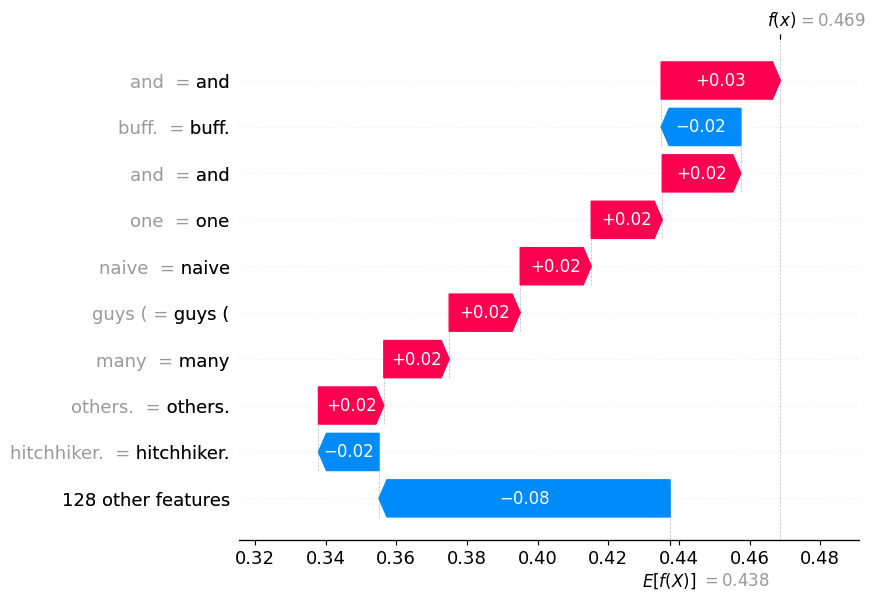
\includegraphics[scale=0.35]{student_local_shap_pos.png}
\caption{\textbf{SHAP} explanation generated by the student model $S_2$ for a positive-class example.}
\label{student_local_shap_pos}
\end{figure}

\clearpage
\onecolumn
\subsection{\textbf{Integrated Gradients} Results}
\label{anexo:ig}

\begin{figure}[h!]
\centering
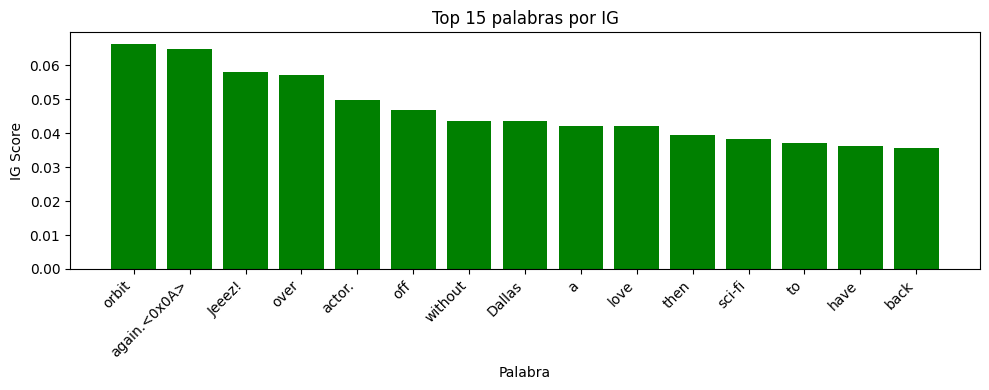
\includegraphics[scale=0.5]{teacher_int_grad_neg.png}
\caption{\textbf{Integrated Gradients} explanation generated by the teacher model $P$ for a negative-class example. The \textit{padding token} was chosen as the baseline for the method.}
\label{teacher_int_grad_neg}
\end{figure}
\begin{figure}[h!]
\centering

\includegraphics[scale=0.5]{student_int_grad_neg.png}
\caption{\textbf{Integrated Gradients} explanation generated by the student model $S_1$ for a negative-class example. The \textit{padding token} was chosen as the baseline for the method.}
\label{student_int_grad_neg}
\end{figure}
\begin{figure}[h!]
\centering
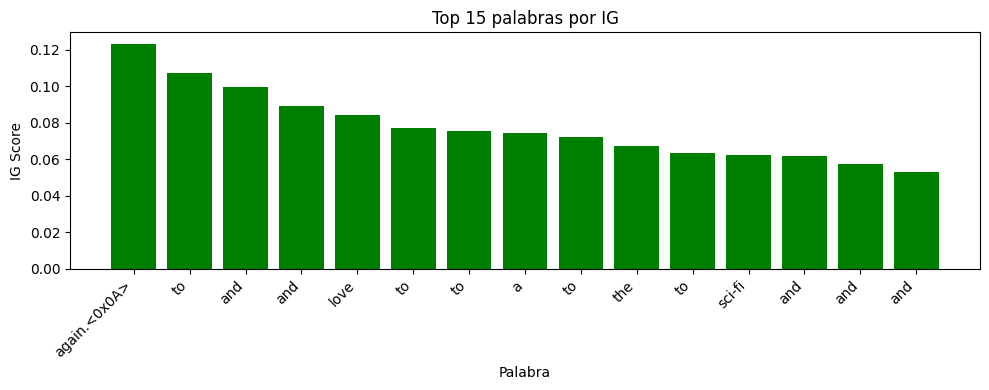
\includegraphics[scale=0.5]{student_local_int_grad_neg.png}
\caption{\textbf{Integrated Gradients} explanation generated by the student model $S_2$ for a negative-class example. The \textit{padding token} was chosen as the baseline for the method.}
\label{student_local_int_grad_neg}
\end{figure}

\begin{figure}[h!]
\centering
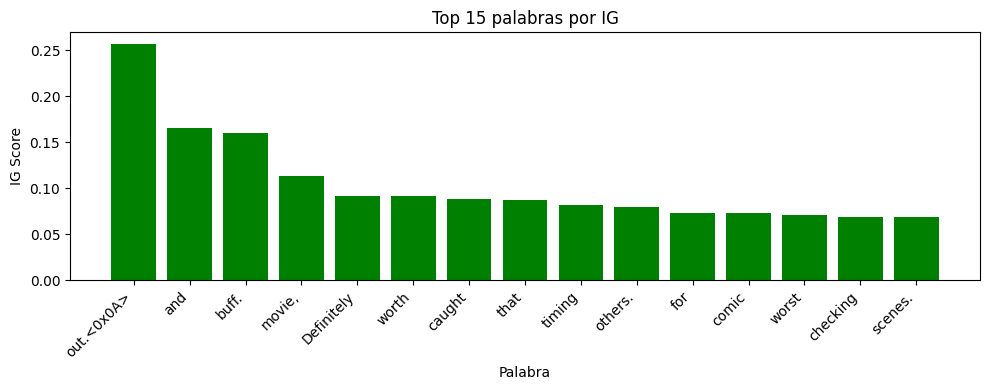
\includegraphics[scale=0.5]{teacher_int_grad_pos.png}
\caption{\textbf{Integrated Gradients} explanation generated by the teacher model $P$ for a positive-class example. The \textit{padding token} was chosen as the baseline for the method.}
\label{teacher_int_grad_pos}
\end{figure}
\begin{figure}[h!]
\centering

\includegraphics[scale=0.5]{student_int_grad_pos.png}
\caption{\textbf{Integrated Gradients} explanation generated by the student model $S_1$ for a positive-class example. The \textit{padding token} was chosen as the baseline for the method.}
\label{student_int_grad_pos}
\end{figure}
\begin{figure}[h!]
\centering
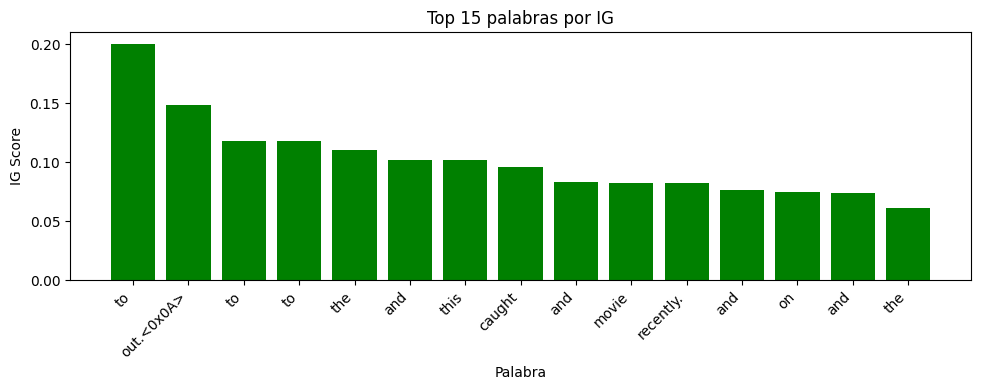
\includegraphics[scale=0.5]{student_local_int_grad_pos.png}
\caption{\textbf{Integrated Gradients} explanation generated by the student model $S_2$ for a positive-class example. The \textit{padding token} was chosen as the baseline for the method.}
\label{student_local_int_grad_pos}
\end{figure}

\twocolumn

\end{document}
